\begin{figure}
    \centering
    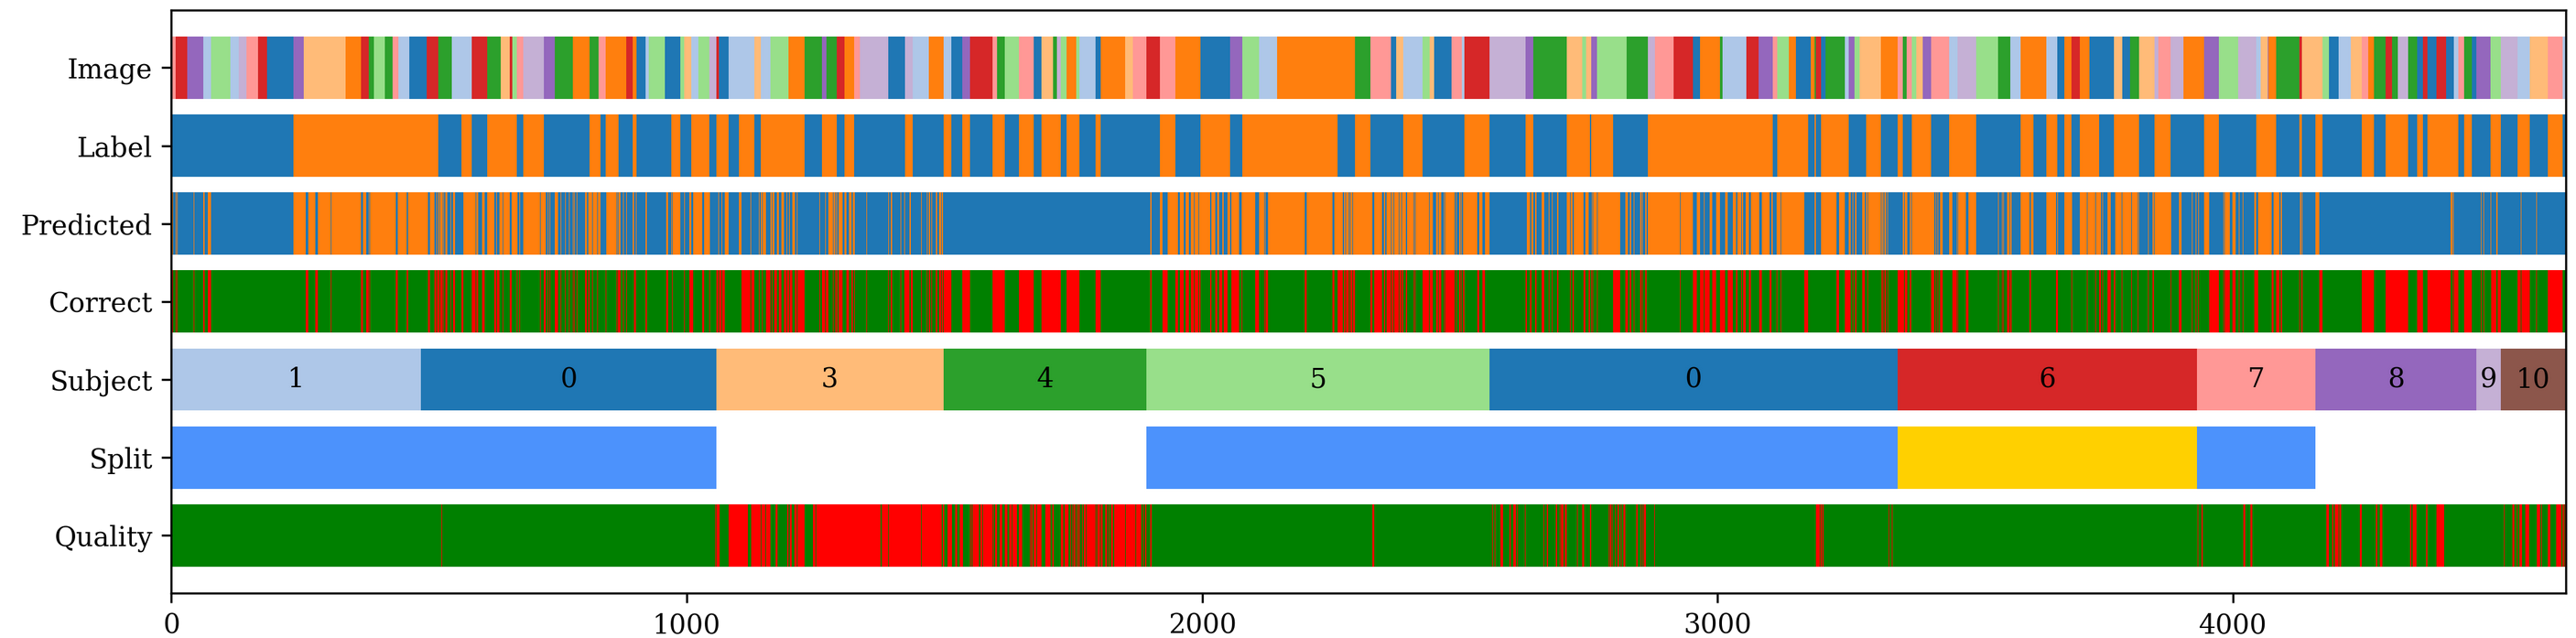
\includegraphics[width=\linewidth]{img/timebars.png}
    \caption{Visualization of the labeled data with classifications from one example subject-fold. Shows the \emph{Image} (stimuli), the class \emph{Label} for that stimuli (\textcolor{NavyBlue}{\textbf{blue}} is code, \textcolor{BurntOrange}{\textbf{orange}} is prose), the \emph{Predicted} class, whether the prediction is \emph{Correct}, the \emph{Subject}, the \emph{Split}/Fold (\textcolor{NavyBlue}{\textbf{blue}} shows the training set, \textcolor{Goldenrod}{\textbf{yellow}} the test set), and our threshold measure for signal \emph{Quality} (\textcolor{Green}{\textbf{green}} indicates acceptable quality). The x-axis is the window index, sorted by acquisition time.
    \\
    \vspace{0.5em}
    It can be seen that (1) subjects \#3 and \#4 have bad signal quality, and have therefore been excluded from the training set. (2) The subjects \#9 and \#10 have also been excluded from training due to issues during data collection. (3) For subject \#1 the stimuli images were not shuffled. (4) Subject \#0 appears twice, as they did two sessions (using unseen stimuli).}\label{fig:timebars}
\end{figure}
